\chapter{\RH\ Algorithm}
\label{chap:Rosu-Havelund Algorithm}

\GRKH\ developed an alternative technique to \Buchi\ automata for evaluating LTL formulae over a trace by using an algorithm they describe in their paper \cite{RosuHavelund}. The algorithm is limited to evaluating formulae specified in the grammar and semantics of the future. Grammar and semantics are given in sections \ref{sec:LTLFutureGrammar} and \ref{sec:LTLFutureSemantics} respectively.

We decided to use this algorithm due to the claim 'that it is hard, if not impossible, to find more efficient algorithms than those presented in this paper'. The low runtime complexity compared to \Buchi\ automata, suggests it is viable for realtime monitoring.

The algorithm operates in two phases: First is an initialisation phase that parses an LTL formula to produce two registers.  The initial phase gets performed once.  The second phase is an evaluation phase, where the formula gets evaluated over a trace. The evaluation phase gets performed for each event in a trace.

\section{Initialisation Phase}
\label{sec:InitialisationPhase}
The intialisation phase produces two registers called \textit{now} and \textit{next}

\begin{description}
\item[Step 1] Produce a subformula tree.\\
\\
A subformula tree is a binary tree where each node is decorated with a formula.  Two nodes are connected if one node has the other as a direct subformula.

\begin{enumerate}
\item A node has either a left and right successor.
\item Or a node has a single left successor.
\item Or a node is a leaf and has no successors.
\end{enumerate}

If the outermost operator is binary then the node's left successor is the first operand and the right successor is the second operand.  If the outermost operator is unary then the left successor is the single operand.  If there are no operators then the formula is a literal and the node has no successors.\\\end{description}

\begin{myEx}
Given a formula such as	$ \varphi = \LTLalways((p \,U q) \rightarrow \LTLeventually(q \rightarrow \LTLnext r)) $ that formula is first transformed to the following subformula tree:\\
\begin{figure}[h]
\centering
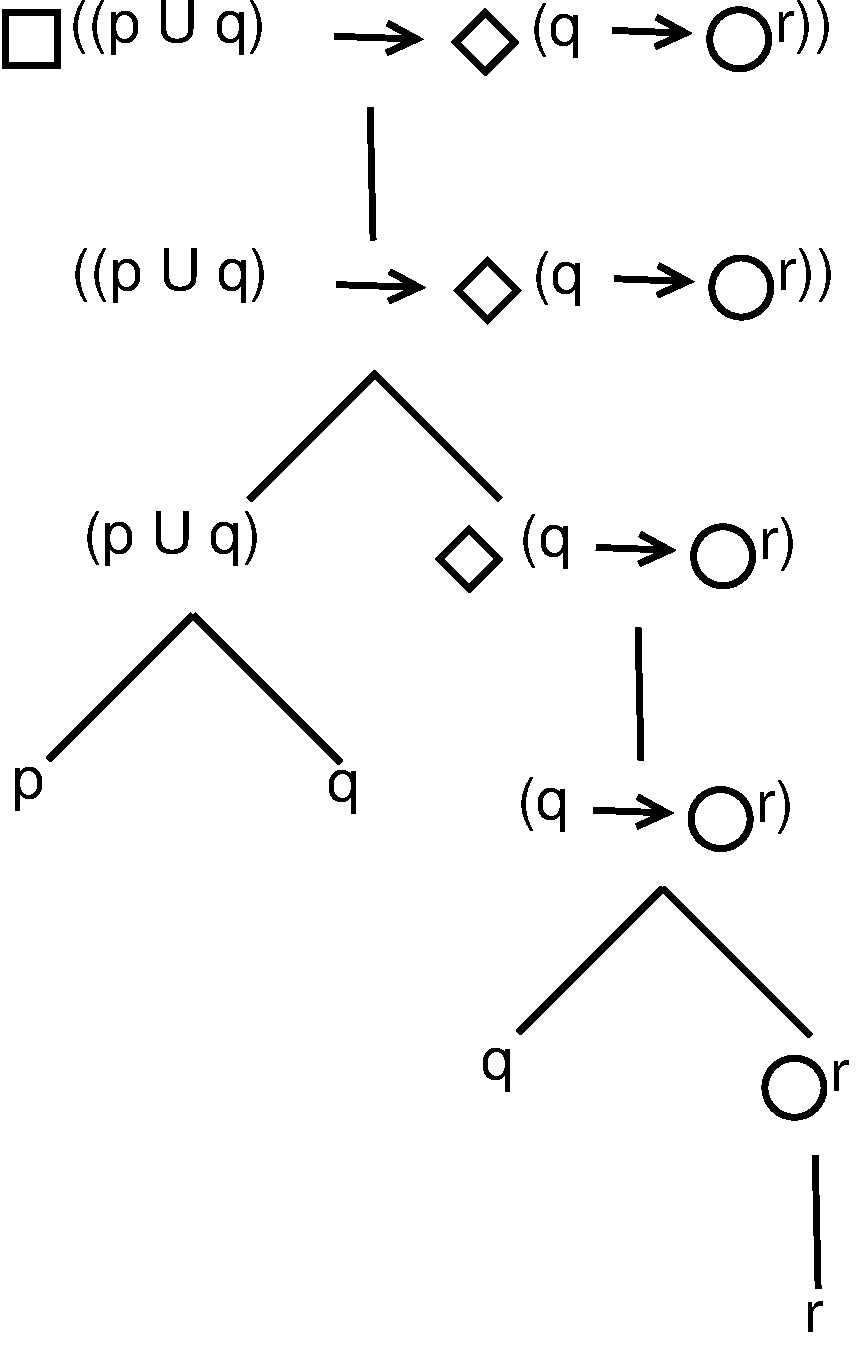
\includegraphics[height=0.3\textheight]{graphics/SubformulaTree}
\label{fig:subformulaTree}
\end{figure}
\\
\qed
\end{myEx}

\begin{description}
\item[Step 2] Walk the tree in breadth-first order to produce a list of subformulae.
\end{description}

\begin{myEx} When we walk the tree in previous example, we get the following subformulae:%The formula $ \varphi = \LTLalways((p \,U q) \rightarrow \LTLeventually(q \rightarrow \LTLnext r)) $ produces subformulae:
\begin{flushleft}
$ \varphi_{1} = \LTLalways((p \,U q) \rightarrow \LTLeventually(q \rightarrow \LTLnext r)) $ \\
$ \varphi_{2} = ((p \,U q) \rightarrow \LTLeventually(q \rightarrow \LTLnext r)) $ \\
$ \varphi_{3} = (p \,U q) $ \\
$ \varphi_{4} = \LTLeventually(q \rightarrow \LTLnext r) $ \\
$ \varphi_{5} = p $ \\
$ \varphi_{6} = q $ \\
$ \varphi_{7} = (q \rightarrow \LTLnext r) $ \\
$ \varphi_{8} = q $ \\
$ \varphi_{9} = \LTLnext r $ \\
$ \varphi_{10} = r $ 
\end{flushleft}
\qed
\end{myEx}

\begin{description}
\item[Step 3] Construct two identical registers called \textit{now} and \textit{next}.  Each register is a one-dimensional array of booleans, where each element corresponds to a formula from the subformulae list, and the length of the array is equal to the length of that list.  Both registers are a permanent breadth-first ordering of the subformula tree.  The first element in the register corresponds to the root of the tree and the last element in the register corresponds to the deepest leaf node of the tree.  The boolean value in each element of the array will hold the truth value that results from evaluating a trace event.\\
\end{description}

\begin{myEx} The now and next registers:\\
\begin{tabular}{cc|c|c|c|c|c|c|c|c|c|c|} &
\multicolumn{1}{c}{} &
\multicolumn{1}{c} {$ \varphi_{1}$} &
\multicolumn{1}{c} {$ \varphi_{2}$} &
\multicolumn{1}{c} {$ \varphi_{3}$} &
\multicolumn{1}{c} {$ \varphi_{4}$} &
\multicolumn{1}{c} {$ \varphi_{5}$} &
\multicolumn{1}{c} {$ \varphi_{6}$} &
\multicolumn{1}{c} {$ \varphi_{7}$} &
\multicolumn{1}{c} {$ \varphi_{8}$} & 
\multicolumn{1}{c} {$ \varphi_{9}$} & 
\multicolumn{1}{c} {$ \varphi_{10}$} \\
\cline{3-12}
& now & $\LTLalways$ & $\rightarrow$ & $U$ & $\LTLeventually$ & $p$ & $q$ & $\rightarrow$ & $q$ & $\LTLnext$ & $r$ \\
\cline{3-12}
\end{tabular}\\
\begin{tabular}{cc|c|c|c|c|c|c|c|c|c|c|} &
\multicolumn{1}{c}{} &
\multicolumn{1}{c} {$ \varphi_{1}$} &
\multicolumn{1}{c} {$ \varphi_{2}$} &
\multicolumn{1}{c} {$ \varphi_{3}$} &
\multicolumn{1}{c} {$ \varphi_{4}$} &
\multicolumn{1}{c} {$ \varphi_{5}$} &
\multicolumn{1}{c} {$ \varphi_{6}$} &
\multicolumn{1}{c} {$ \varphi_{7}$} &
\multicolumn{1}{c} {$ \varphi_{8}$} & 
\multicolumn{1}{c} {$ \varphi_{9}$} & 
\multicolumn{1}{c} {$ \varphi_{10}$} \\
\cline{3-12}
& next & $\LTLalways$ & $\rightarrow$ & $U$ & $\LTLeventually$ & $p$ & $q$ & $\rightarrow$ & $q$ & $\LTLnext$ & $r$ \\
\cline{3-12}
\end{tabular}\\
\qed
\end{myEx}

\begin{description}
\item[Step 4] Before the evaluation phase is performed, the truth values of the \textit{next} register must be initialised.  Traverse the register from the last cell to the first, the initial truth value of the element is the value arrived at when evaluating the subformula over an empty trace ($ \epsilon $).  The semantics are those of the future LTL operators and are given in definition \ref{def:FutureEmptyTraceSemantics}.\\
\end{description}

\begin{myEx} Given the example formula $ \varphi = \LTLalways((p \,U q) \rightarrow \LTLeventually(q \rightarrow \LTLnext r))$ the first cell to be initialised is the cell corresponding to $ \varphi_{10}$, which is the literal r in the subformula tree.  According to semantic rule 1 defined in \ref{def:FutureEmptyTraceSemantics}, a literal over the empty trace evaluates to $ \bot $.  Therefore, after the first cell is evaluated the \textit{next} register looks as follows:

\begin{tabular}{cc|c|c|c|c|c|c|c|c|c|c|} &
\multicolumn{1}{c}{} &
\multicolumn{1}{c} {$ \varphi_{1}$} &
\multicolumn{1}{c} {$ \varphi_{2}$} &
\multicolumn{1}{c} {$ \varphi_{3}$} &
\multicolumn{1}{c} {$ \varphi_{4}$} &
\multicolumn{1}{c} {$ \varphi_{5}$} &
\multicolumn{1}{c} {$ \varphi_{6}$} &
\multicolumn{1}{c} {$ \varphi_{7}$} &
\multicolumn{1}{c} {$ \varphi_{8}$} & 
\multicolumn{1}{c} {$ \varphi_{9}$} & 
\multicolumn{1}{c} {$ \varphi_{10}$} \\
\cline{3-12}
& next & $\LTLalways$ & $\rightarrow$ & $U$ & $\LTLeventually$ & $p$ & $q$ & $\rightarrow$ & $q$ & $\LTLnext$ & $\bot$ \\
\cline{3-12}
\end{tabular}\\
\\
\\
The second cell to be initialised is $\varphi_{9}$, the formula $\LTLnext r$.  Rule 6 says the next operator evaluates to $ \bot $ over the empty trace:

\begin{tabular}{cc|c|c|c|c|c|c|c|c|c|c|} &
\multicolumn{1}{c}{} &
\multicolumn{1}{c} {$ \varphi_{1}$} &
\multicolumn{1}{c} {$ \varphi_{2}$} &
\multicolumn{1}{c} {$ \varphi_{3}$} &
\multicolumn{1}{c} {$ \varphi_{4}$} &
\multicolumn{1}{c} {$ \varphi_{5}$} &
\multicolumn{1}{c} {$ \varphi_{6}$} &
\multicolumn{1}{c} {$ \varphi_{7}$} &
\multicolumn{1}{c} {$ \varphi_{8}$} & 
\multicolumn{1}{c} {$ \varphi_{9}$} & 
\multicolumn{1}{c} {$ \varphi_{10}$} \\
\cline{3-12}
& next & $\LTLalways$ & $\rightarrow$ & $U$ & $\LTLeventually$ & $p$ & $q$ & $\rightarrow$ & $q$ & $\bot$ & $\bot$ \\
\cline{3-12}
\end{tabular}\\
\\
\\
The next cell to be initialised is $\varphi_8$, another literal, therefore it takes the value $\bot$:

\begin{tabular}{cc|c|c|c|c|c|c|c|c|c|c|} &
\multicolumn{1}{c}{} &
\multicolumn{1}{c} {$ \varphi_{1}$} &
\multicolumn{1}{c} {$ \varphi_{2}$} &
\multicolumn{1}{c} {$ \varphi_{3}$} &
\multicolumn{1}{c} {$ \varphi_{4}$} &
\multicolumn{1}{c} {$ \varphi_{5}$} &
\multicolumn{1}{c} {$ \varphi_{6}$} &
\multicolumn{1}{c} {$ \varphi_{7}$} &
\multicolumn{1}{c} {$ \varphi_{8}$} & 
\multicolumn{1}{c} {$ \varphi_{9}$} & 
\multicolumn{1}{c} {$ \varphi_{10}$} \\
\cline{3-12}
& next & $\LTLalways$ & $\rightarrow$ & $U$ & $\LTLeventually$ & $p$ & $q$ & $\rightarrow$ & $\bot$ & $\bot$ & $\bot$ \\
\cline{3-12}
\end{tabular}\\
\\
\\
The formula corresponding to cell $\varphi_7$ is $(q \rightarrow \LTLnext r)$.  The semantics of the implies operator are defined by rule 5: The cell takes the value of $\top$ when the antecedent is $\bot$.  In this case the antecedent is the literal q and the corresponding cell, $\varphi_8$, evaluated to $\bot$ in the previous step.  Therefore $\varphi_7$ takes the value $\top$ because the antecedent evaluates to $ \bot $.  The \textit{next} register is updated to look like:

\begin{tabular}{cc|c|c|c|c|c|c|c|c|c|c|} &
\multicolumn{1}{c}{} &
\multicolumn{1}{c} {$ \varphi_{1}$} &
\multicolumn{1}{c} {$ \varphi_{2}$} &
\multicolumn{1}{c} {$ \varphi_{3}$} &
\multicolumn{1}{c} {$ \varphi_{4}$} &
\multicolumn{1}{c} {$ \varphi_{5}$} &
\multicolumn{1}{c} {$ \varphi_{6}$} &
\multicolumn{1}{c} {$ \varphi_{7}$} &
\multicolumn{1}{c} {$ \varphi_{8}$} & 
\multicolumn{1}{c} {$ \varphi_{9}$} & 
\multicolumn{1}{c} {$ \varphi_{10}$} \\
\cline{3-12}
& next & $\LTLalways$ & $\rightarrow$ & $U$ & $\LTLeventually$ & $p$ & $q$ & $\top$ & $\bot$ & $\bot$ & $\bot$ \\
\cline{3-12}
\end{tabular}\\
\\
\\
This process continues until all the cells of the \textit{next} register have been initialised by evaluation over the empty trace.  The cells in the \textit{now} register are written to by the second phase of the algorithm before they are read, therefore they do not require any initialisation.\\
\\
When the process is complete the two registers appear as follows:\\
\noindent
\begin{tabular}{cc|c|c|c|c|c|c|c|c|c|c|} &
\multicolumn{1}{c}{} &
\multicolumn{1}{c} {$ \varphi_{1}$} &
\multicolumn{1}{c} {$ \varphi_{2}$} &
\multicolumn{1}{c} {$ \varphi_{3}$} &
\multicolumn{1}{c} {$ \varphi_{4}$} &
\multicolumn{1}{c} {$ \varphi_{5}$} &
\multicolumn{1}{c} {$ \varphi_{6}$} &
\multicolumn{1}{c} {$ \varphi_{7}$} &
\multicolumn{1}{c} {$ \varphi_{8}$} & 
\multicolumn{1}{c} {$ \varphi_{9}$} & 
\multicolumn{1}{c} {$ \varphi_{10}$} \\
\cline{3-12}
& next & $\top$ & $\top$ & $\bot$ & $\top$ & $\bot$ & $\bot$ & $\top$ & $\bot$ & $\bot$ & $\bot$\\
\cline{3-12}
\end{tabular}\\
\\
\begin{tabular}{cc|c|c|c|c|c|c|c|c|c|c|} &
\multicolumn{1}{c}{} &
\multicolumn{1}{c} {$ \varphi_{1}$} &
\multicolumn{1}{c} {$ \varphi_{2}$} &
\multicolumn{1}{c} {$ \varphi_{3}$} &
\multicolumn{1}{c} {$ \varphi_{4}$} &
\multicolumn{1}{c} {$ \varphi_{5}$} &
\multicolumn{1}{c} {$ \varphi_{6}$} &
\multicolumn{1}{c} {$ \varphi_{7}$} &
\multicolumn{1}{c} {$ \varphi_{8}$} & 
\multicolumn{1}{c} {$ \varphi_{9}$} & 
\multicolumn{1}{c} {$ \varphi_{10}$} \\
\cline{3-12}
& now & $\LTLalways$ & $\rightarrow$ & $U$ & $\LTLeventually$ & $p$ & $q$ & $\rightarrow$ & $q$ & $\LTLnext$ & $r$ \\
\cline{3-12}
\end{tabular}\\
\\
\qed
\end{myEx}
\noindent That concludes the first phase of the algorithm that produces two registers from an LTL formula.\\  

\section{Evaluation Phase}
\label{sec:EvaluationPhase}
The second phase of the algorithm evaluates the formula over a non-empty trace and is performed for every event in the trace.\\
\begin{description}
%\item[Step 1] When a new event occurs add that event to the end of the trace.

\item[Step 1] Traverse the trace from the last entry to the first, taking each entry from the trace.  With that entry traverse the \textit{now} register from last cell to the first, evaluating the corresponding subformula over the trace entry, according to the operator's semantics from definition \ref{def:FutureNon-emptyTraceSemantics}.  Set the boolean value of the cell to the resulting truth value.

\item[Step 2] next[i] = now[i] for all i ranging from 1..length(now).

\item[Step 3] Repeat steps 2 and 3 with the preceding (earlier) trace entry until arriving at the head of the trace where there is no preceding entry.

\item[Step 4] The final result of evaluating the formula over the trace is found as the truth value of the first cell in the \textit{next} register because this cell corresponds to the root of the subformula tree.\\
\end{description}

Understanding steps 1 and 2 is key to understanding the \RH\ algorithm and how it evaluates the temporal operators of LTL.  There are three elements to understanding these steps, the \textit{next} register, the relation between the \textit{now} register and the \textit{next} register and the order that the trace is evaluated.

To explain how to evaluate a trace event in relation to the registers, we have to adapt the semantics from definition \ref{def:FutureNon-emptyTraceSemantics} to refer to the registers.  We replace $e$ with a reference to the \textit{now} register and $t$ becomes the \textit{next} register.  The subformulae of $ \varphi $ are replaced with references to the corresponding cells within the \textit{now} and \textit{next} registers by the use of indices $i$, $j$, and $k$.  The index $i$ maps to the cell corresponding to the subformula's operator.  Indices $j$ and $k$ map to the cells corresponding to the left and right operands respectively.  The registers are ordered breadth-first, so an operator comes before it's operands in a register, thus $i < j < k$.\\
%The semantics described below are used in step 1 when evaluating a subformula.  They are an adaptation of the semantics found in definition \ref{def:FutureNon-emptyTraceSemantics} but e t is replaced with a reference to the \textit{now} register and t becomes the \textit{next} register.  The subformulae of $ \varphi $ are replaced with references to the corresponding cells within the \textit{now} and \textit{next} registers by the use of indices i, j, and k.  The index i maps to the cell corresponding to the subformulas operator, while indexes j and k map to the cells corresponding to the left and right operands of the subformula respectively.  The registers are a breadth-first ordering of the subformula tree, therefore an operator comes before its operands in a register, thus i $ < $ j and i $ < $ k.\\
\\
For a given trace event $e$, for all $i$ ranging from length(\textit{now})..1, if the $i^{th}$ outermost operator is:
\begin{enumerate}
\item literal l, then \textit{now}[$i$] $ \leftarrow $ (l == $e$)
\item $ \neg $ then \textit{now}[$i$] $ \leftarrow $ NOT(\textit{now}[$j$]).
\item $ \lor $ then \textit{now}[$i$] $ \leftarrow $ \textit{now}[$j$] OR \textit{now}[$k$]. 
\item $ \land $ then \textit{now}[$i$] $ \leftarrow $ \textit{now}[$j$] AND \textit{now}[$k$]. 
\item $ \rightarrow $ then now[$i$] $ \leftarrow $ NOT(\textit{now}[$j$]) OR \textit{now}[$k$]. 
\item $ \LTLnext $ then \textit{now}[$i$] $ \leftarrow $ \textit{next}[$j$].
\item $ \LTLalways $ then \textit{now}[$i$] $ \leftarrow $ \textit{now}[$j$] AND \textit{next}[$i$].
\item $ \LTLeventually $ then \textit{now}[$i$] $ \leftarrow $ \textit{now}[$j$] OR \textit{next}[$i$].
\item U then \textit{now}[$i$] $ \leftarrow $ \textit{now}[$k$] OR (\textit{now}[$j$] AND \textit{next}[$i$]).
\end{enumerate}

The reader may notice that the boolean operators $ \neg, \lor, \land, \rightarrow $ only reference other cells in the \textit{now} register.  This is because the semantics of these operators do not depend on any other events within the trace.  Whereas the semantics of the temporal operators $ \LTLnext, \ \LTLalways,  \ \LTLeventually, \ U $ depend on events that may have occurred elsewhere in the trace so they also reference the \textit{next} register.

The \textit{next} register represents the cumulative evaluations of all trace events after the event currently being evaluated.  Following each evaluation of an event, the cells of the \textit{next} register get set to the corresponding values from the \textit{now} register.  But we can see that evaluation of the \textit{now} register is itself based upon the earlier state of the \textit{next} register.  This circular-referencing process accumulates all prior evaluations into the \textit{next} register.  Because the trace gets evaluated from the latest entry to the earliest, those prior evaluations are all the events that occurred after the current event.  Therefore the evaluation of each event in the trace is based upon the prior evaluation of events that come after.

Evaluating events from latest to earliest explains why the algorithm is limited to implementing only the future LTL operators; when evaluating an event only the evaluations of `future' events are known.

\begin{myEx}
Example evaluation of a trace $t$ that satisfies $ \varphi $
\\*
$ t = \langle p, q, r \rangle $\\
$ \varphi = \LTLeventually((p \,U q) \rightarrow \LTLeventually(q \rightarrow \LTLnext r)) $\\

\textbf{\item[Phase 1] Initialisation}\\
\\
\begin{tabular}{cc|c|c|c|c|c|c|c|c|c|c|} &
\multicolumn{1}{c}{} &
\multicolumn{1}{c} {$ \varphi_{1}$} &
\multicolumn{1}{c} {$ \varphi_{2}$} &
\multicolumn{1}{c} {$ \varphi_{3}$} &
\multicolumn{1}{c} {$ \varphi_{4}$} &
\multicolumn{1}{c} {$ \varphi_{5}$} &
\multicolumn{1}{c} {$ \varphi_{6}$} &
\multicolumn{1}{c} {$ \varphi_{7}$} &
\multicolumn{1}{c} {$ \varphi_{8}$} & 
\multicolumn{1}{c} {$ \varphi_{9}$} & 
\multicolumn{1}{c} {$ \varphi_{10}$} \\
\cline{3-12}
& next & $ \top $ & $ \top $ & $ \bot $ & $ \top $ & $ \bot $ & $ \bot $ & $ \top $ & $ \bot $ & $ \bot $ & $ \bot $ \\
\cline{3-12}
\end{tabular}\\
\\
\begin{tabular}{cc|c|c|c|c|c|c|c|c|c|c|} &
\multicolumn{1}{c}{} &
\multicolumn{1}{c} {$ \varphi_{1}$} &
\multicolumn{1}{c} {$ \varphi_{2}$} &
\multicolumn{1}{c} {$ \varphi_{3}$} &
\multicolumn{1}{c} {$ \varphi_{4}$} &
\multicolumn{1}{c} {$ \varphi_{5}$} &
\multicolumn{1}{c} {$ \varphi_{6}$} &
\multicolumn{1}{c} {$ \varphi_{7}$} &
\multicolumn{1}{c} {$ \varphi_{8}$} & 
\multicolumn{1}{c} {$ \varphi_{9}$} & 
\multicolumn{1}{c} {$ \varphi_{10}$} \\
\cline{3-12}
& now & $\LTLalways$ & $\rightarrow$ & $U$ & $\LTLeventually$ & $p$ & $q$ & $\rightarrow$ & $q$ & $\LTLnext$ & $r$ \\
\cline{3-12}
\end{tabular}\\
\\
\textbf{\item[Phase 2] Evaluation}\\
\subitem \underline{Iteration 1, e = r}
\\
\\
\noindent The evaluation phase begins with the \textit{next} register as below:

\begin{tabular}{cc|c|c|c|c|c|c|c|c|c|c|} &
\multicolumn{1}{c}{} &
\multicolumn{1}{c} {$ \varphi_{1}$} &
\multicolumn{1}{c} {$ \varphi_{2}$} &
\multicolumn{1}{c} {$ \varphi_{3}$} &
\multicolumn{1}{c} {$ \varphi_{4}$} &
\multicolumn{1}{c} {$ \varphi_{5}$} &
\multicolumn{1}{c} {$ \varphi_{6}$} &
\multicolumn{1}{c} {$ \varphi_{7}$} &
\multicolumn{1}{c} {$ \varphi_{8}$} & 
\multicolumn{1}{c} {$ \varphi_{9}$} & 
\multicolumn{1}{c} {$ \varphi_{10}$} \\
\cline{3-12}
& next & $ \top $ & $ \top $ & $ \bot $ & $ \top $ & $ \bot $ & $ \bot $ & $ \top $ & $ \bot $ & $ \bot $ & $ \bot $ \\
\cline{3-12}
\end{tabular}\\
\\
\\
The first cells to be evaluated correspond to subformulae $\varphi_{10}$ down to $\varphi_{5}$, according to rules 1, 5 and 6 from section \ref{sec:EvaluationPhase} these only reference other cells in the \textit{now} register and evaluate as follows:

\begin{tabular}{cc|c|c|c|c|c|c|c|c|c|c|} &
\multicolumn{1}{c}{} &
\multicolumn{1}{c} {$ \varphi_{1}$} &
\multicolumn{1}{c} {$ \varphi_{2}$} &
\multicolumn{1}{c} {$ \varphi_{3}$} &
\multicolumn{1}{c} {$ \varphi_{4}$} &
\multicolumn{1}{c} {$ \varphi_{5}$} &
\multicolumn{1}{c} {$ \varphi_{6}$} &
\multicolumn{1}{c} {$ \varphi_{7}$} &
\multicolumn{1}{c} {$ \varphi_{8}$} & 
\multicolumn{1}{c} {$ \varphi_{9}$} & 
\multicolumn{1}{c} {$ \varphi_{10}$} \\
\cline{3-12}
& now & $\LTLalways$ & $\rightarrow$ & $U$ & $\LTLeventually$ & $ \bot $ & $ \bot $ & $ \top $ & $ \bot $ & $ \top $ & $ \top $ \\
\cline{3-12}
\end{tabular}\\
\\
\\
The $now[4]$ cell corresponds to the subformula $\LTLeventually(q \rightarrow \LTLnext r)$.  Rule 8 defines the semantics of the eventually operator $\LTLeventually$.  The \textit{next} register is required because eventually formulae take the value $ \top $ when the subformula is either true now, or some time in the future.  Therefore $now[4]$ is $ \top $ if $now[7]$ or $next[4]$ is $\top$.  In this case the cell evaluates to $\top$ and the \textit{now} register is updated to appear:

\begin{tabular}{cc|c|c|c|c|c|c|c|c|c|c|} &
\multicolumn{1}{c}{} &
\multicolumn{1}{c} {$ \varphi_{1}$} &
\multicolumn{1}{c} {$ \varphi_{2}$} &
\multicolumn{1}{c} {$ \varphi_{3}$} &
\multicolumn{1}{c} {$ \varphi_{4}$} &
\multicolumn{1}{c} {$ \varphi_{5}$} &
\multicolumn{1}{c} {$ \varphi_{6}$} &
\multicolumn{1}{c} {$ \varphi_{7}$} &
\multicolumn{1}{c} {$ \varphi_{8}$} & 
\multicolumn{1}{c} {$ \varphi_{9}$} & 
\multicolumn{1}{c} {$ \varphi_{10}$} \\
\cline{3-12}
& now & $\LTLalways$ & $\rightarrow$ & $U$ & $\top$ & $ \bot $ & $ \bot $ & $ \top $ & $ \bot $ & $ \top $ & $ \top $ \\
\cline{3-12}
\end{tabular}\\
\\
\\
The $\varphi_{3}$ cell corresponds to the formula $p \,U q$ which is the until temporal operator.  Rule 9 applies to the until operator.  It evaluates $\top$ when the left operand, p, is true now or the right operand, q, is true now and the whole subformula is true in the future.  The cell evaluates $\bot$.

\begin{tabular}{cc|c|c|c|c|c|c|c|c|c|c|} &
\multicolumn{1}{c}{} &
\multicolumn{1}{c} {$ \varphi_{1}$} &
\multicolumn{1}{c} {$ \varphi_{2}$} &
\multicolumn{1}{c} {$ \varphi_{3}$} &
\multicolumn{1}{c} {$ \varphi_{4}$} &
\multicolumn{1}{c} {$ \varphi_{5}$} &
\multicolumn{1}{c} {$ \varphi_{6}$} &
\multicolumn{1}{c} {$ \varphi_{7}$} &
\multicolumn{1}{c} {$ \varphi_{8}$} & 
\multicolumn{1}{c} {$ \varphi_{9}$} & 
\multicolumn{1}{c} {$ \varphi_{10}$} \\
\cline{3-12}
& now & $\LTLalways$ & $\rightarrow$ & $ \bot $ & $ \top $ & $ \bot $ & $ \bot $ & $ \top $ & $ \bot $ & $ \bot $ & $ \top $ \\
\cline{3-12}
\end{tabular}\\
\\
\\
The $\varphi_{2}$ cell is the implies formula $(p \,U q) \rightarrow \LTLeventually(q \rightarrow \LTLnext r)$.  By Rule 5 the cell evaluates to $\top$.

\begin{tabular}{cc|c|c|c|c|c|c|c|c|c|c|} &
\multicolumn{1}{c}{} &
\multicolumn{1}{c} {$ \varphi_{1}$} &
\multicolumn{1}{c} {$ \varphi_{2}$} &
\multicolumn{1}{c} {$ \varphi_{3}$} &
\multicolumn{1}{c} {$ \varphi_{4}$} &
\multicolumn{1}{c} {$ \varphi_{5}$} &
\multicolumn{1}{c} {$ \varphi_{6}$} &
\multicolumn{1}{c} {$ \varphi_{7}$} &
\multicolumn{1}{c} {$ \varphi_{8}$} & 
\multicolumn{1}{c} {$ \varphi_{9}$} & 
\multicolumn{1}{c} {$ \varphi_{10}$} \\
\cline{3-12}
& now & $\LTLalways$ & $ \top $ & $ \bot $ & $ \top $ & $ \bot $ & $ \bot $ & $ \top $ & $ \bot $ & $ \bot $ & $ \top $ \\
\cline{3-12}
\end{tabular}\\
\\
\\
The final cell $ \varphi_{1}$ is the third temporal operator of the formula, the always operator.  By Rule 7 the cell evaluates to $\top $ when the subformula is $\top$ now and $\top$ for all following trace entries.  Therefore evaluation of this formula is the conjunction of $now[2]$ with $next[1]$.  It takes the value $\top$.

\begin{tabular}{cc|c|c|c|c|c|c|c|c|c|c|} &
\multicolumn{1}{c}{} &
\multicolumn{1}{c} {$ \varphi_{1}$} &
\multicolumn{1}{c} {$ \varphi_{2}$} &
\multicolumn{1}{c} {$ \varphi_{3}$} &
\multicolumn{1}{c} {$ \varphi_{4}$} &
\multicolumn{1}{c} {$ \varphi_{5}$} &
\multicolumn{1}{c} {$ \varphi_{6}$} &
\multicolumn{1}{c} {$ \varphi_{7}$} &
\multicolumn{1}{c} {$ \varphi_{8}$} & 
\multicolumn{1}{c} {$ \varphi_{9}$} & 
\multicolumn{1}{c} {$ \varphi_{10}$} \\
\cline{3-12}
& now & $ \top $  & $ \top $ & $ \bot $ & $ \top $ & $ \bot $ & $ \bot $ & $ \top $ & $ \bot $ & $ \bot $ & $ \top $ \\
\cline{3-12}
\end{tabular}\\
\\
\\
\noindent Once the \textit{now} register has been evaluated the values in the \textit{next} register are overwritten with those from the \textit{now} register and it appears as:

\begin{tabular}{cc|c|c|c|c|c|c|c|c|c|c|} &
\multicolumn{1}{c}{} &
\multicolumn{1}{c} {$ \varphi_{1}$} &
\multicolumn{1}{c} {$ \varphi_{2}$} &
\multicolumn{1}{c} {$ \varphi_{3}$} &
\multicolumn{1}{c} {$ \varphi_{4}$} &
\multicolumn{1}{c} {$ \varphi_{5}$} &
\multicolumn{1}{c} {$ \varphi_{6}$} &
\multicolumn{1}{c} {$ \varphi_{7}$} &
\multicolumn{1}{c} {$ \varphi_{8}$} & 
\multicolumn{1}{c} {$ \varphi_{9}$} & 
\multicolumn{1}{c} {$ \varphi_{10}$} \\
\cline{3-12}
& next & $ \top $  & $ \top $ & $ \bot $ & $ \top $ & $ \bot $ & $ \bot $ & $ \top $ & $ \bot $ & $ \bot $ & $ \top $ \\
\cline{3-12}
\end{tabular}\\
\\
\\
\subitem \underline{Iteration 2, e = q}

\begin{tabular}{cc|c|c|c|c|c|c|c|c|c|c|} &
\multicolumn{1}{c}{} &
\multicolumn{1}{c} {$ \varphi_{1}$} &
\multicolumn{1}{c} {$ \varphi_{2}$} &
\multicolumn{1}{c} {$ \varphi_{3}$} &
\multicolumn{1}{c} {$ \varphi_{4}$} &
\multicolumn{1}{c} {$ \varphi_{5}$} &
\multicolumn{1}{c} {$ \varphi_{6}$} &
\multicolumn{1}{c} {$ \varphi_{7}$} &
\multicolumn{1}{c} {$ \varphi_{8}$} & 
\multicolumn{1}{c} {$ \varphi_{9}$} & 
\multicolumn{1}{c} {$ \varphi_{10}$} \\
\cline{3-12}
& next & $ \top $ & $ \top $ & $ \bot $ & $ \top $ & $ \bot $ & $ \bot $ & $ \top $ & $ \bot $ & $ \bot $ & $ \top $ \\
\cline{3-12}
\end{tabular}\\

\begin{tabular}{cc|c|c|c|c|c|c|c|c|c|c|} &
\multicolumn{1}{c}{} &
\multicolumn{1}{c} {$ \varphi_{1}$} &
\multicolumn{1}{c} {$ \varphi_{2}$} &
\multicolumn{1}{c} {$ \varphi_{3}$} &
\multicolumn{1}{c} {$ \varphi_{4}$} &
\multicolumn{1}{c} {$ \varphi_{5}$} &
\multicolumn{1}{c} {$ \varphi_{6}$} &
\multicolumn{1}{c} {$ \varphi_{7}$} &
\multicolumn{1}{c} {$ \varphi_{8}$} & 
\multicolumn{1}{c} {$ \varphi_{9}$} & 
\multicolumn{1}{c} {$ \varphi_{10}$} \\
\cline{3-12}
& now & $ \top $ & $ \top $ & $ \top $ & $ \top $ & $ \bot $ & $ \top $ & $ \top $ & $ \top $ & $ \top $ & $ \bot $ \\
\cline{3-12}
\end{tabular}\\
\\
\\
\subitem \underline{Iteration 3, e = p}

\begin{tabular}{cc|c|c|c|c|c|c|c|c|c|c|} &
\multicolumn{1}{c}{} &
\multicolumn{1}{c} {$ \varphi_{1}$} &
\multicolumn{1}{c} {$ \varphi_{2}$} &
\multicolumn{1}{c} {$ \varphi_{3}$} &
\multicolumn{1}{c} {$ \varphi_{4}$} &
\multicolumn{1}{c} {$ \varphi_{5}$} &
\multicolumn{1}{c} {$ \varphi_{6}$} &
\multicolumn{1}{c} {$ \varphi_{7}$} &
\multicolumn{1}{c} {$ \varphi_{8}$} & 
\multicolumn{1}{c} {$ \varphi_{9}$} & 
\multicolumn{1}{c} {$ \varphi_{10}$} \\
\cline{3-12}
& next & $ \top $ & $ \top $ & $ \top $ & $ \top $ & $ \bot $ & $ \top $ & $ \top $ & $ \top $ & $ \top $ & $ \bot $ \\
\cline{3-12}
\end{tabular}\\

\begin{tabular}{cc|c|c|c|c|c|c|c|c|c|c|} &
\multicolumn{1}{c}{} &
\multicolumn{1}{c} {$ \varphi_{1}$} &
\multicolumn{1}{c} {$ \varphi_{2}$} &
\multicolumn{1}{c} {$ \varphi_{3}$} &
\multicolumn{1}{c} {$ \varphi_{4}$} &
\multicolumn{1}{c} {$ \varphi_{5}$} &
\multicolumn{1}{c} {$ \varphi_{6}$} &
\multicolumn{1}{c} {$ \varphi_{7}$} &
\multicolumn{1}{c} {$ \varphi_{8}$} & 
\multicolumn{1}{c} {$ \varphi_{9}$} & 
\multicolumn{1}{c} {$ \varphi_{10}$} \\
\cline{3-12}
& now & $ \top $ & $ \top $ & $ \top $ & $ \top $ & $ \top $ & $ \bot $ & $ \top $ & $ \bot $ & $ \bot $ & $ \bot $ \\
\cline{3-12}
\end{tabular}\\
\\
\\
\subitem \underline{Final state}

\begin{tabular}{cc|c|c|c|c|c|c|c|c|c|c|} &
\multicolumn{1}{c}{} &
\multicolumn{1}{c} {$ \varphi_{1}$} &
\multicolumn{1}{c} {$ \varphi_{2}$} &
\multicolumn{1}{c} {$ \varphi_{3}$} &
\multicolumn{1}{c} {$ \varphi_{4}$} &
\multicolumn{1}{c} {$ \varphi_{5}$} &
\multicolumn{1}{c} {$ \varphi_{6}$} &
\multicolumn{1}{c} {$ \varphi_{7}$} &
\multicolumn{1}{c} {$ \varphi_{8}$} & 
\multicolumn{1}{c} {$ \varphi_{9}$} & 
\multicolumn{1}{c} {$ \varphi_{10}$} \\
\cline{3-12}
& next & $ \top $ & $ \top $ & $ \top $ & $ \top $ & $ \top $ & $ \bot $ & $ \top $ & $ \bot $ & $ \bot $ & $ \bot $ \\
\cline{3-12}
\end{tabular}\\
\\
\\
$ t \models \varphi = next[1] = \top $
\qed
\end{myEx}

This concludes our description of how the \RH\ algorithm operates.


